\documentclass{article}
\usepackage{mathtools}
\usepackage{pgf}
\usepackage{tikz}
\usetikzlibrary{arrows,automata}

\begin{document}
\section{Introduction}
Many of the useful properties of the Fourier transform arise because it diagonalises translation.
More precisely, it expresses a function $f$ in the form
\[
f(x) = \frac{1}{\sqrt{2\pi}}\int_{-\infty}^\infty F(\omega)\exp(i\omega x)d\omega
\]
i.e. as a kind of linear combination of functions $x\rightarrow\exp(i\omega x)$.
These functions have the property that under translation they are multiplied by $i\omega$.
This gives a representation of functions that behaves particularly simply under translations.
It also gives a representation of functions that behaves well with a wide variety of other operations such as differentiation, integration and convolution.
These operations can be thought of as being conceptually built from translations.
For example differentiation is a bit like subtracting a function from its infinitesimal translate.

The $n$-dimensional Fourier transform gives a nice representation of functions in $n$ variables where we're interested in operations related to translations in $n$-dimensions.

The translations form a Lie group.
What about different groups like the rotations in 3D, $SO(3)$?
This group is non-commutative so we can't expect non-trivial diagonal representations.
But we can start with one axis, say the $z$-axis, and start by diagoinalising with respect to just the rotations around that axis.
If we use the usual coordinates $x$, $y$ and $z$ in 3D then we can write functions of $x$, $y$, and $z$ as functions of polar coordinates $r$, $\theta$ and $\phi$ where
\begin{align*}
x & = & r\cos(\phi)\sin(\theta) \\
y & = & r\sin(\phi)\sin(\theta) \\
z & = & r\cos(\theta) \\
\end{align*}
For integer $m$, any function $f$ of the form $f(r,\theta,\phi) = g(r,\theta)\exp(im\phi)$ is multiplied by a constant when rotated around the $z$-axis.
We can then seek to find functions $g$ that make $f$ as well behaved as possible when rotated around the other axes.
A good choice turns out to be the spherical harmonics.

Now consider another group: the Euclidean group $E(2)$ consisting of rotations and translations in the plane.
Can we find a family of functions that is well behaved under the action of this group?

\section{Partially diagonalising $E(2)$}
$E(2)$ is not commutative so we can't expect to completely diagonalise it.
Let's start by defining 2D polar coordinates by
\begin{align*}
x & = & r\cos(\theta) \\
y & = & r\sin(\theta) \\
\end{align*}
Now consider functions of the form $f_m(r,\theta)=b_m(r)\exp(im\theta)$.
This mimics how the spherical harmonics work with $SO(3)$ and are clearly very well behaved with respect to rotations around the origin.
Write $R(\phi)$ for such a rotation by angle $\phi$.
Then 
\[
(R(\phi)f)(x,y) = f(x,y)\exp(-im\phi).
\]
So now we need to pick functions $b_m$ that behave nicely under translation.
We can make our life easier by focusing on infinitesimal translations.
So let's pick $b_n$ so that the $f_m$ take a particularly simple form when differentiated.
For convenience also define $z=x+iy$.

Differentiating and simplifying we get both
\[
\frac{\partial f_n}{\partial x} = 
    \Big(-\frac{inyb_n(r)}{r}+xb_n'(r)\Big)\exp(i(n+1)\theta)
\]
and
\[
\frac{\partial f_n}{\partial y} = 
    \Big(-\frac{inxb_n(r)}{r}+yb_n'(r)\Big)\exp(i(n+1)\theta)
\]
This is a little messy.
But there's a trick to simplify.
We have $x$ and $y$ appearing in different places in both of the right hand sides, but by forming $\partial f_n/\partial x+i\partial f_n/\partial y$ they both become multiples of $z$ which can be factored out.
We could do the same using $-i$ instead.
We get both:
\[
\frac{\partial f_n}{\partial x}+i\frac{\partial f_n}{\partial y} =
    \Big(-\frac{nb_n(r)}{r}+b_n'(r)\Big)\exp(i(n+1)\theta)
\]
and
\[
\frac{\partial f_n}{\partial x}-i\frac{\partial f_n}{\partial y} =
    \Big(\frac{nb_n(r)}{r}+b_n'(r)\Big)\exp(i(n-1)\theta)
\]

We're interested in functions of the form
$f_n(r,\theta)=b_n(r)\exp(im\theta)$
and these become particularly nice if we choose
\begin{align*}
b_{n+1}(r) & = & -\frac{nb_n(r)}{r}+b_n'(r) \\
b_{n-1}(r) & = & \frac{nb_n(r)}{r}+b_n'(r) \\
\end{align*}
or equivalently
(XXX I got opposite of this. Redo.)
\begin{align}
\frac{2b_n(r)}{r} & = & b_{n-1}(r)+b_{n+1}(r) \label{sum} \\
2b_n'(r) & = & b_{n-1}(r)-b_{n+1}(r) \label{deriv}
\end{align}
Any family of functions $b_n$ satisfying these properties will result in the simple relations:
\[
\frac{\partial f_n}{\partial x}+i\frac{\partial f_n}{\partial y} =
    f_{n+1}(x,y)
\]
and
\[
\frac{\partial f_n}{\partial x}-i\frac{\partial f_n}{\partial y} =
    f_{n-1}(x,y).
\]

\section{Exponentiating up to translation}
By Equation~(\ref{deriv}) we can collect up all of the recurrence relations for the derivatives of the $b_n$ as
\[
\begin{pmatrix}
\vdots \\
b'_{-1}(x) \\
\boxed{b'_0(x)} \\
b'_1(x) \\
\vdots \\
\end{pmatrix}
=
M
\begin{pmatrix}
\vdots \\
b_{-1}(x) \\
\boxed{b_0(x)} \\
b_1(x) \\
\vdots \\
\end{pmatrix}
\]
where
\[
M=\frac{1}{2}
\begin{pmatrix*}[r]
\ddots & \ddots &   &    &   &   &        \\
\ddots & \hphantom{-{}}1 & 0 & -1 &   &   &        \\
       &   & \phantom{-{}}1 & \boxed{0} & -1 &   &        \\
       &   &   & 1 & 0 & -1 & \ddots \\
       &   &   &   &   & \ddots & \ddots \\
\end{pmatrix*}.
\]
These are vectors and a matrix that are infinite in both directions so I've used a box to indicate the $0$-th and $(0,0)$-th elements.

I'm calling any family of functions $(b_i)$ satisfying a relation of this type a \textit{family of Bessel type}.

In general we have
\[
f(x+a) = f(x)+f'(x)a+f''(x)a^2/2+f^{(3)}(x)a^3/3!+\ldots
\]
which we can write succinctly as the ``shift rule''
\[
\exp(aD)f(x) = f(x+a).
\]
where $D=d/dx$.
For our vector of $b_i$'s we can represent $D$ as $M$.
Se we have
\[
b_i(x+a) = \exp(aM)b_i(x).
\]
So we now have to exponentiate $aM$.

We can view that matrix as the transition matrix for the non-deterministic automaton in Figure~\ref{automaton} with states labelled $\ldots, -1, 0, 1, \ldots$ and such that it emits a $1$ every time it takes a step to the left and a $-1$ every time it takes a step to the ight.

\begin{figure}
\centering
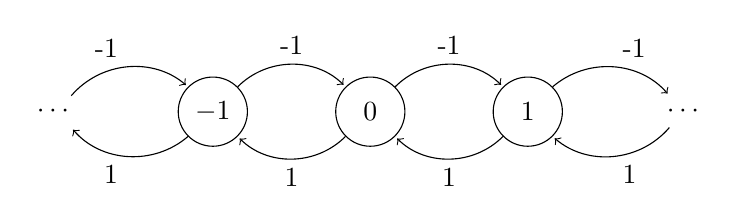
\begin{tikzpicture}[shorten >=1pt,node distance=2cm,auto,bend angle=45]
\node[state]          (q_0)                      {$0$};
\node[state]          (q_-1) [left of =q_0] {$-1$};
\node[]          (q_-2) [left of=q_-1] {$\cdots$};
\node[state]          (q_1) [right of=q_0] {$1$};
\node[]          (q_2) [right of=q_1] {$\cdots$};
\path[->]
          (q_-2)  edge [bend left] node        {-1} (q_-1) 
          (q_-1)  edge [bend left] node        {-1} (q_0) 
          (q_0)   edge [bend left] node        {-1} (q_1) 
          (q_1)   edge [bend left] node        {-1} (q_2)
          (q_2)  edge [bend left] node        {1} (q_1) 
          (q_1)  edge [bend left] node        {1} (q_0) 
          (q_0)   edge [bend left] node        {1} (q_-1) 
          (q_-1)   edge [bend left] node        {1} (q_-2);
\end{tikzpicture}
\caption{An automaton}
\label{automaton}
\end{figure}
With that in mind, the $(i,j)$th element of $M^n$ is the number of ways to take a path from $i$ to $j$ in $n$ steps but counting with a weight of $(-1)^R$ for paths that take $R$ steps to the right.
I.e.
\[
(M^n)_{ij} = \sum_{P:\mbox{$n$ step paths $i\rightarrow j$}} (-1)^{R(P)}\Big(\frac{1}{2}\Big)^n
\]
If the number of steps left for a path is $L$ then $j-i=R-L$ and $L+R=n$.
So as a function of $L$, the number of steps in a path is $n=j-i+L$.
The terms in $\exp(aM)$ sums over all paths of any length, but with paths of length $n$ weighted by $\frac{1}{n!}$.
\[
\exp(aM)_{ij} = \sum_{P:\mbox{paths }i\rightarrow j} \frac{1}{n(P)!}(-1)^{R(P)} (\frac{a}{2})^{n(P)}
\]
There are $\binom{n}{L}=\binom{j-i+2L}{L}$ ways to pick a path with $n$ steps that moves left $L$ times.
\[
b_i(x+a) = \sum_{j=-\infty}^\infty\sum_{L=0}^\infty\frac{(-1)^{j-i+L}}{L!(j-i+L)!}(\frac{a}{2})^{j-i+2L} b_j(x)
\]
Any $(b_i)$ that satisfies this property will satisfy Equations~(\ref{sum}) and (\ref{deriv}).
Given our freedom of choice we may as well pick $b_j(0)=\delta_{j0}$ giving us
\[
b_i(a) = \sum_{L=0}^\infty\frac{(-1)^{-i+L}}{L!(-i+L)!}(\frac{a}{2})^{-i+2L} .
\]
There's another way to sumover these weighted paths.
When expanding $(t+t^{-1})^n$, the coefficient of $t^m$ is the number of paths with $n$ steps that end up $m$ positions to the right.
Similarly the coefficient of $t^m$ in $(t-t^{-1})^n$ is the weighted count with weight equal to $(-1)^{\mbox{$\#$ of right steps in path}}$.
The coefficient
\[
\exp(a(t-t^{-1})/2)
\]

\end{document}
